\chapter{Improving flexibility of macros}\label{sect:flex}
\label{improving-flexibility-macros}

% \todo[inline]{Explain the old macro system with an example. Q: Isn't that the section below already?}

% \section{Explanation of the macro system}
\section{The macro system}
% What are the limitations without macros?
% Most importantly: syncats. gf-ud assumes that every word is in a leaf, represented by a lexical gf-function. however, syncategorimatic words \todo{define?} (or functions?) come from the functions that are used to combine trees (what are those called?) and would be missing otherwise. E.g. "is" is syncategorimatic in gf for english, because there is no lexical function for copula, because not all languages use a word for copula. So we make up a lexical gf-function for "is", which is then combined with a made-up version of MkCl which is converted into the thing we need.
% This is terrible writing!

% Motivate need for auxfuns and auxcats

GF trees are on a higher abstraction level than UD trees. In UD, every token is associated with a dependency label. In contrast, any production rule in a GF grammar may introduce new tokens. This difference complicates the mapping between the two formalisms.

In order to overcome some limitations of the conversion from UD to GF, especially the issue with multiple possible matching trees mentioned in \autoref{sec:multiple_trees}, there is a system of macros. A macro is an imaginary GF function that will get converted into an expression of real GF functions after the main conversion step of gf2ud is done.

The full syntax of macros can be found in \autoref{app:annotation}.

% Syncats?
% \todo[inline]{Talk about syncategorematic words}
\subsection{Example 1: \texttt{\#auxfun} and matching morphological features}

When one GF function corresponds to multiple different dependency labels, a macro can be used to disambiguate which one is meant and to avoid losing the information of that distinction.

For example, the GF grammar contains two ways of building a noun phrase without a determiner:
%For example, if we have a noun without a determiner, the algorithm would try all possible ways to build a noun phrase out of it:
an indefinite plural, using \verb|DetCN aPl_Det : CN -> NP|\footnote{Becuase the \texttt{aPl\_Det} function does not correspond to a word, the algorithm would actually not try to construct it.}, or mass noun, using \verb|MassNP : CN -> NP|.
% \verb|DetCN aPl_Det : CN -> NP|
% IndefPlNP : CN -> NP
Knowing which function to choose is trivial for a human reader, because we see it from the form of the word: \emph{water} in ``I drink \emph{water}'' is a singular mass noun, and \emph{children} in ``\emph{Children} are playing'' is an indefinite plural. But for the ud2gf algorithm, this is impossible with the tools we have seen so far. %tricky to do with just abstract annotations.

The annotation scheme introduced in \autoref{sec:annotations-intro} operates on abstract syntax only, and thus it has no way to distinguish between those cases, because it has no information about concrete morphological features.
% In order to create mass noun phrases of singular nouns and plural noun phrases of plural nouns,

In order to choose the right function depending on features beyond the dependency label, the macros can also match against part of speech and morphological features using the syntax \verb|dependency_label[Feature=Value]|. Using this syntax, we can make macros for distinguishing between mass nouns and indefinite plurals:

\begin{lstlisting}
    -- disable plurals as mass terms
    #disable MassNP
    #auxfun MassNP_sg cn : CN -> NP = MassNP        cn ; head[Number=Sing]
    #auxfun DetCN_aPl cn : CN -> NP = DetCN aPl_Det cn ; head[Number=Plur]
\end{lstlisting}

In order to ensure that the macros are used instead of the original functions, we first \verb|#disable| all the original functions that might get applied too liberally (in this case, only \verb|MassNP|).
Next we create macros that check for the correct number of the noun before constructing a noun phrase.
% Notice that the macro \verb|DetCN_aPl| combines the syntactic function \verb|DetCN : Det -> CN -> NP| with the lexical function \verb|aPl_Det : Det|.

Let's consider the sentence ``Children are playing'', and what would happen to it if we didn't force mass nouns and indefinite plurals to be introduced via macros.

The algorithm from \autoref{sec:overview-of-algorithm} goes through each word\footnote{Remember that all the words are parsed into a lexical category, which is determined by the \texttt{\#cat} annotation.}, and tries all possible functions that can be applied to them.
However, \verb|MassNP| is the only function we can apply to the word \emph{child}: the algorithm would never apply the correct \verb|DetCN aPl_Det| without a macro, because the lexical function \verb|aPl_Det| does not correspond to any word, and thus would be never introduced into the tree.

So the two macros fill two purposes: preventing \verb|MassNP| from being applied too liberally, and making \verb|DetCN aPl_Det| possible in the first place.

Note that none of this would be a problem, if the original phrase had a determiner. If the sentence were instead ``Many children are playing'', then the NP formed by \verb|MassNP| would still be formed, but discarded as soon as the algorithm enters the next step and tries to combine the noun and the determiner.

%If we have available \verb|MassNP : CN -> NP|, that tree is built every single time we have a CN available.
%If the original phrase had a determiner, like ``Many children are playing'', then the NP formed by \verb|MassNP| is discarded as soon as the algorithm enters the next step and tries to combine the noun and the determiner.
%But now that the phrase has no determiner in the first place, the algorithm could pick the \verb|MassNP| version, instead of the correct indefinite plural. And in fact, the algorithm would never build the correct \verb|DetCN aPl_Det| form without this macro, because the lexical function \verb|aPl_Det| does not correspond to any word, so it was never introduced into the tree.

\subsection{Example 2: \texttt{\#auxcat} and syncategorematic words}

%Another common case when macros are needed are so-called \emph{syncategorematic} words:
Another common use case for macros is to handle so-called \emph{syncategorematic} words.
Syncategorematic words are words that are introduced as a part of the linearization of some syntactic function, and don't have a GF category or function of their own.


% In the GF grammar, the string \emph{is} or \emph{are} is produced by \verb|UseAP|, as a way to convert an AP into a VP.

% that are associated with non-lexical functions\footnote{A lexical function is a function that takes zero arguments, which means that it will be in a leaf of the tree.}. For example, in GF, the copula is syncategorematic, which means that they cannot be parsed on their own using GF.

When introducing the problem and its partial solution, in \cite{kolachina-ranta-2017} \citeauthor{kolachina-ranta-2017} name as examples copulas, negations, tense auxiliaries and infinitive marks. We reproduce their example of the English copula (the verb ``to be'') and its treatment in \verb|ud2gf|.

Figures \ref{fig:gf-this-cat-is-small} and \ref{fig:ud-this-cat-is-small} show the difference between GF's and UD's treatment of copulas. In the UD tree, the copula has a category and a dependency label \verb|cop|. In the GF tree, there is no special category: the string ``is'' is introduced by the function \verb|UseAP : AP -> VP| rule, which makes an AP into a predicate.

\begin{figure}
    \centering
    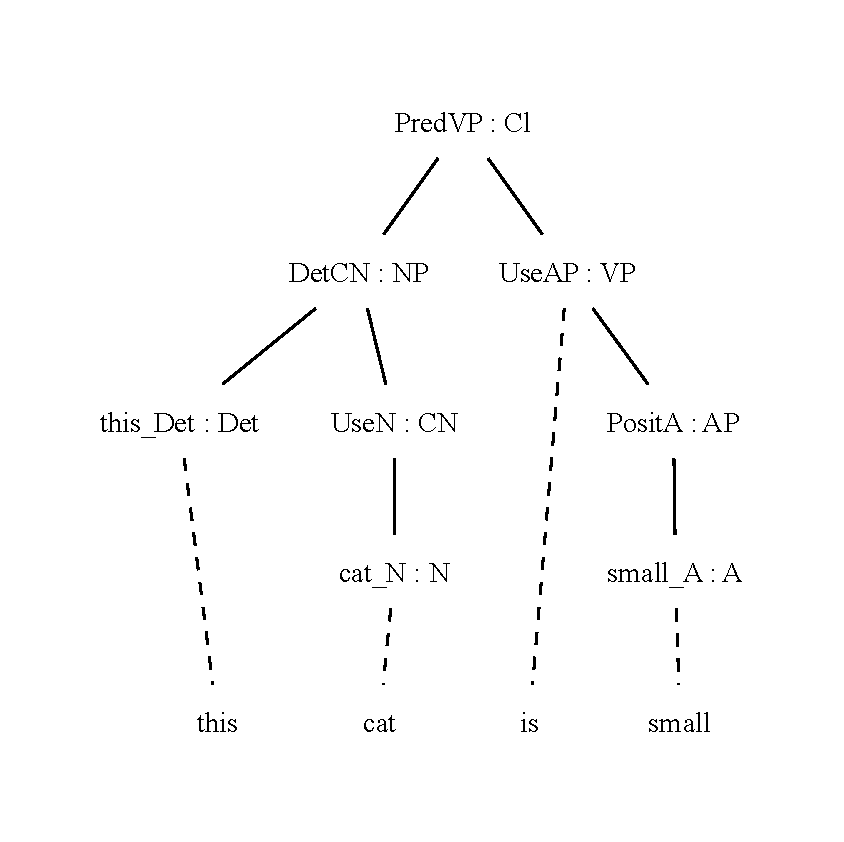
\includegraphics{figure/thiscatissmall.pdf}
    \caption{The phrase ``This cat is small'' analysed as a GF tree.}
    \label{fig:gf-this-cat-is-small}
% Generated using:
% > p -cat=Cl "this cat is small"  | ? grep -v '["?]'
% > pt PredVP (DetCN (DetQuant this_Quant NumSg) (UseN cat_N)) (UseComp (CompAP (PositA small_A)))  | vp -format=pdf -showfun
% on the UDApp grammar
\end{figure}


% result from \verb+p -cat=Cl "this cat is small"  | vp -view=open -showfun+:

% Produced using: https://maryszmary.github.io/ud-annotatrix//standalone/annotator.html
% And pressing the printer icon to select latex

\begin{figure}
    \centering
    % \includegraphics{}
    \begin{dependency}
       \begin{deptext}[column sep=0.4cm]
             this \& cat \& is \& small \\
           {\tt DET}\&{\tt NOUN}\&{\tt AUX}\&{\tt ADJ}\\
       \end{deptext}
       \depedge{2}{1}{det}
       \depedge{4}{2}{nsubj}
       \depedge{4}{3}{cop}
    \end{dependency} \\
    \caption{The phrase ``This cat is small'' analysed as a UD tree.}
    \label{fig:ud-this-cat-is-small}
\end{figure}

As a solution, \verb|ud2gf| introduced the notion of \emph{auxiliary categories} and auxiliary functions.
% This consists of the following parts:
This time we use the following auxiliary category and auxiliary function:
\begin{itemize}
    \item Auxiliary category for copula: \verb|#auxcat Cop VERB|. This annotation introduces an auxiliary category \texttt{Cop} and associates it with the UD part of speech \texttt{VERB}.
    \item Auxiliary function (macro) that recognises the auxiliary category: \\
          \verb|  #auxfun UseAP_ cop ap : Cop -> AP -> VP = UseAP ap ; cop head|. \\
          The macro takes a copula and an adjectival phrase and then throws away the copula, because the copula (\emph{is}) is created by the \texttt{UseAP} function.
    \item A declaration of the lemma \emph{be}: \\ \verb|  #lemma DEFAULT_ be Cop cop head|. \\
    Here we declare that the lemma can be used with all functions (\verb|DEFAULT_|), the lemma is \emph{be}, the auxiliary category should be \emph{Cop}, the dependency label pointing at the lemma should be \emph{cop} and that the \emph{head} argument of the function should be the parent of the copula. Most parts of the \verb|#lemma| declaration are only used for the gf2ud direction. Only the lemma name and category name are used by ud2gf.
\end{itemize}
% #lemma DEFAULT_ be Cop cop head


% #lemma <functions> <lemma> <category> <own label> <target label>

% \begin{itemize}
%     \item
%     \item
%     % \item Rule to replace the auxiliary function with an actual GF function: \\
%     %       \verb|  #auxfun UseAP_ cop ap = UseAP ap|
% \end{itemize}

However, coordination was still a problem in \verb|ud2gf|. The auxiliary categories and functions were not expressive enough to transform a structure like ``the small, cute and fluffy cat'' from UD to GF.

\FloatBarrier

\section{Problem: Limitations of the possible tree transformation}

As an example of a phrase that can be difficult to convert using the old ud2gf, let us consider the adjectival phrase ``small, furry, fluffy and cute''
would be described in UD format as in \autoref{fig:ud_cute}.


% \begin{figure}
%     \begin{verbatim}
%     1  cute  cute  ADJ  JJ  Degree=Pos  0  root  _  FUN=cute_A
%     2  ,  ,  PUNCT  ,  _  3  punct  _  _
%     3  fluffy  fluffy  ADJ  JJ  Degree=Pos  1  conj  _  FUN=fluffy_A
%     4  and  and  CCONJ  CC  _  5  cc  _  FUN=and_Conj
%     5  furry  furry  ADJ  JJ  Degree=Pos  1  conj  _  FUN=furry_A
%     \end{verbatim}
%     % \begin{tabular}{|c|c|c|c|c|c|c|c|c|c|}
%     % \hline
%     % 1 & cute & cute & ADJ & JJ & Degree\=Pos & 0 & root & \_ & FUN\=cute\_A \
%     % \hline
%     % 2 & , & , & PUNCT & , & \_ & 3 & punct & \_ & \_ \
%     % \hline
%     % 3 & fluffy & fluffy & ADJ & JJ & Degree\=Pos & 1 & conj & _ & FUN\=fluffy\_A \
%     % \hline
%     % 4 & and & and & CCONJ & CC & \_ & 5 & cc & \_ & FUN\=and\_Conj \
%     % \hline
%     % 5 & furry & furry & ADJ & JJ & Degree\=Pos & 1 & conj & \_ & FUN\=furry\_A \
%     % \hline
%     % \end{tabular}
%     \caption{The phrase ``small, furry, fluffy and cute'' as a textual UD tree}
%     \label{fig:ud_cute_text}
% \end{figure}

\begin{figure}
    \centering
    % \begin{dependency}
  \begin{deptext}[column sep=0.4cm]
      cute \& , \& fluffy \& and \& furry \\
    {\tt ADJ}\&{\tt PUNCT}\&{\tt ADJ}\&{\tt CCONJ}\&{\tt ADJ} \\
  \end{deptext}
  \depedge{2}{1}{punct}
  \depedge{0}{2}{conj}
  \depedge{4}{3}{cc}
  \depedge{0}{4}{conj}
\end{dependency} \\
    % \includesvg{ud-annotatrix-corpus.svg}
    % 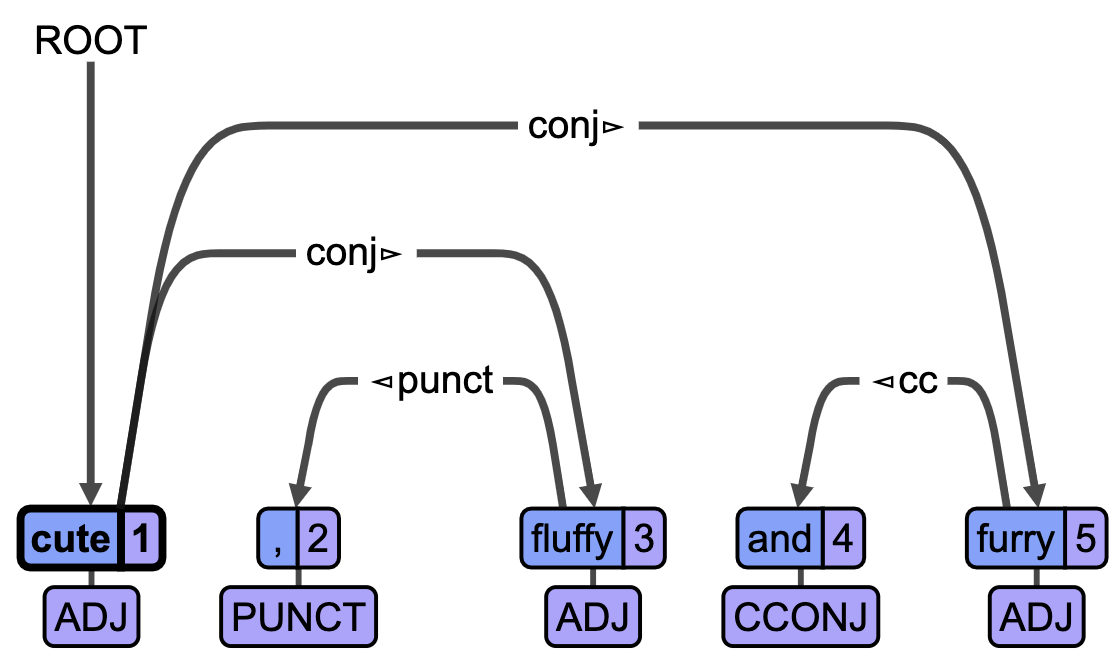
\includegraphics[width=0.7\textwidth]{figure/ud_cute.png}
    \begin{dependency}
        \begin{deptext}[column sep=0.4cm]
              small \& , \& furry \&  , \& fluffy \& and \& cute \\
            {\tt ADJ}\&{\tt PUNCT}\&{\tt ADJ}\&{\tt PUNCT}\&{\tt ADJ}\&{\tt CCONJ}\&{\tt ADJ}\\
        \end{deptext}
        \depedge{3}{2}{punct}
        \depedge{1}{3}{conj}
        \depedge{5}{4}{punct}
        \depedge{1}{5}{conj}
        \depedge{7}{6}{cc}
        \depedge{1}{7}{conj}
    \end{dependency} \\
    \caption{The phrase ``small, furry, fluffy and cute'' as a UD tree in graphical format}
    \label{fig:ud_cute}
\end{figure}
% \include{}

\begin{figure}
    \centering
    % \begin{dependency}
  \begin{deptext}[column sep=0.4cm]
      cute \& , \& fluffy \& and \& furry \\
    {\tt ADJ}\&{\tt PUNCT}\&{\tt ADJ}\&{\tt CCONJ}\&{\tt ADJ} \\
  \end{deptext}
  \depedge{2}{1}{punct}
  \depedge{0}{2}{conj}
  \depedge{4}{3}{cc}
  \depedge{0}{4}{conj}
\end{dependency} \\
    % \includesvg{ud-annotatrix-corpus.svg}
    % 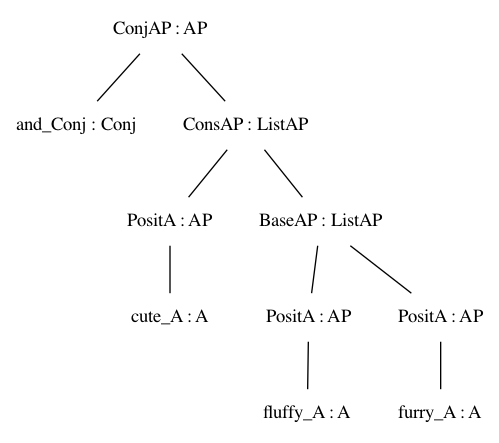
\includegraphics[width=0.7\textwidth]{figure/cute_gf.png}
    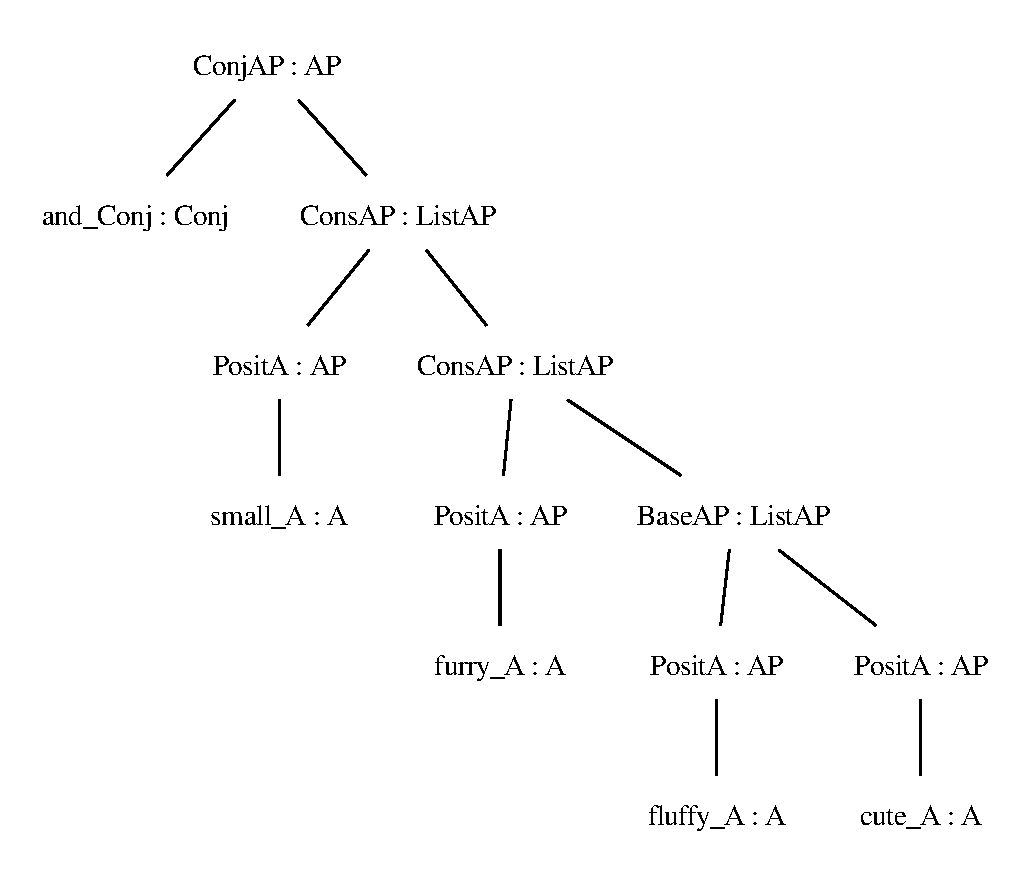
\includegraphics[width=0.7\textwidth]{figure/cute_gf.eps}
    % Generated with
    % vt -format=eps ConjAP and_Conj (ConsAP (PositA small_A) (ConsAP (PositA furry_A) (BaseAP (PositA fluffy_A) (PositA cute_A))))
    % on the UDApp.pgf grammar
    \caption{The phrase ``small, furry, fluffy and cute'' as a GF tree in graphical format.}
    \label{fig:gf_cute}
\end{figure}

The GF version of the same tree, would look like in \autoref{fig:gf_cute}.

% \begin{verbatim}
% ConjAP and_Conj (ConsAP (PositA cute_A)
%                         (BaseAP (PositA fluffy_A) (PositA furry_A)))
% \end{verbatim}

Here we can see that in UD, the word ``cute'' is in the root, while the conjunction ``and'' is at the bottom of the tree, while in GF the conjunction is a direct child of the root. This transformation can not be preformed by the simple single-layer transformations that were available in the old macro-system.

The main issue that made it impossible for the old macros to perform this transformation is that we need to extract several pieces of information from a node and then use them independently.

\section{Solution: Recursive macros}

% Most of the time the structure in UD trees are similar enough to allow a fairly direct translation.
% There are however some difficult cases where the structure is significantly different in a way that was impossible to overcome using the old macro system.
%
% One such example is when you have a series of conjunctions, for example the phrase:
%
%
%   small, fluffy, furry and cute
%
% In

In order to improve the ability to create structurally different trees when converting from UD to GF, the ability for macros to be recursive was added.
This means that when a macro is substituted, the resulting head is checked again to see if the result is another macro, until no more substitutions are possible.
This makes it possible to encode data using Church encoding, in particular the Church encoding for pairs: a higher order function that takes a binary function as an argument and provides the two items it contains to the inner function.
This construction of pairs can also be interpreted as continuation-passing style, where instead of constructing a pair, we take a continuation which would consume the two arguments of the pair.

\begin{verbatim}
type Pair a b = forall c. (a -> b -> c) -> c
\end{verbatim}

In order to construct and consume these pairs we use the following helper functions:
\begin{lstlisting}
-- The syntax of macros type signatures does not allow higher order
-- functions types, so we use the following abbreviations:
-- ab2r = a -> b -> r
-- Pair_a_b = ab2r -> r
#auxfun MkPair_ a b handler : a -> b -> ab2r -> r = handler a b ; head dummy dummy
#auxfun UsePair_ handler pair : ab2r -> Pair_a_b -> r = pair handler ; head dummy
\end{lstlisting}
When using these helpers, you would partially apply the \verb|MkPair_| helper, so it can later get the final \verb|handler| argument from \verb|UsePair_|\footnote{The \texttt{UsePair\_} helper is not strictly necessary, since it can be replaced with function application (\texttt{UsePair\_ handler pair = pair handler}), but it helps making the code clearer. The \texttt{MkPair\_} on the other hand is necessary, because we need to partially apply it.}.
Because the helpers are only used by other macros, we don't need any real dependency labels but instead use dummy values to fill them in (here \texttt{dummy}, but anything would work).


% \begin{lstlisting}
% #auxfun AndCuteCont_ and cute : Conj -> AP -> Pair_Conj_AP = MkPair_ and cute ; cc head
% \end{lstlisting}

In addition to pairs, we will also need triples, which work similarly:
\begin{lstlisting}
-- Triple_a_b_c = (a -> b -> r) -> r
#auxfun MkTriple_ a b c handler : a -> b -> c -> abc2r -> r = handler a b c ; head dummy dummy dummy
#auxfun UseTriple_ handler triple : abc2r -> Triple_a_b_c -> r = triple handler ; head dummy
\end{lstlisting}

As can be seen in \autoref{fig:ud_cute}, each word but the first and last in a coordinate structure has a comma as a dependent in UD. This macro handles that.
\begin{lstlisting}
#auxcat Comma PUNCT
#lemma DEFAULT_ , Comma punct head
#auxfun CommaAP_ ap comma : AP -> Comma -> APComma = ap ; head punct
\end{lstlisting}

The last word has the conjunction as a child in UD, while the conjunction in GF abstract syntax is inserted at the very top, as can be seen in \autoref{fig:gf_cute}. This is where we first use our \verb|MkPair_| helper in order to carry along the last word and the conjunction separately.
\begin{lstlisting}
#auxfun AndCuteCont_ and cute : Conj -> AP -> Pair_Conj_AP = MkPair_ and cute ; cc head
\end{lstlisting}
% TODO: Make names here match the figure
% TODO: Maybe make a larger picture

Because lists in GF have a minimum length of two, we need two base cases: one with exactly two conjuncts and one with three or more.

% Here we have the case
The simplest case is when we only have two words with a conjunction in between (``small and cute'').
The two functions below handle this case.
% We need to handle this case separately because lists in GF have a minimum length of two.

\begin{lstlisting}
#auxfun AP2_ small andCute : AP -> Pair_Conj_AP -> AP = UsePair_ (AP2_helper_ small) andCute ; head conj
#auxfun AP2_helper_ small and cute :  AP -> Conj -> AP -> AP = ConjAP and (BaseAP small cute) ; head dummy dummy
\end{lstlisting}
We need a separate \verb|AP2_helper_| function to handle the extra argument \texttt{small} because we don't have support for lambdas or closures. We can see that the main function \verb|AP2_| gets both parts of the pair ``and cute'' as a bundle, while the \verb|AP2_helper_| gets them as separate arguments.

The next case is when we have at least three conjuncts with a conjunction (``small, fluffy and cute''). Here we need to create a triple, with:
\begin{itemize}
    \item the conjunction (``and'')
    \item the first word in the coordination, which is also the head of the UD tree (``small'')
    \item the two last conjuncts (``fluffy'' and ``cute'') which form base of the GF list (\verb|BaseAP fluffy cute|).
\end{itemize}
\begin{lstlisting}
#auxfun APBaseComma_ small fluffy andCute : AP -> APComma -> Pair_Conj_AP -> ConjListAP = UsePair_ (APBaseComma_helper_ small fluffy) andCute ; head conj conj
#auxfun APBaseComma_helper_ small fluffy and cute : AP -> APComma -> Conj -> AP -> ConjListAP = MkTriple_ and small (BaseAP fluffy cute) ; head dummy dummy
\end{lstlisting}

The next case is for four or more conjuncts with a conjunction (``small, furry, fluffy and cute''). Here we deconstruct the triple, add the middle word (``furry'') to the list (\verb|ConsAP furry (BaseAP fluffy cute)|) and reconstruct the triple.
\begin{lstlisting}
#auxfun APAddComma_ furry and_small_fluffyCute  : APComma -> ConjListAP -> ConjListAP = UseTriple_ (APAddComma_helper_ furry) and_small_fluffyCute ; conj head
#auxfun APAddComma_helper_ furry and small fluffyCute : APComma -> Conj -> AP -> ListAP -> ConjListAP = MkTriple_ and small (ConsAP furry fluffyCute) ; dummy head
\end{lstlisting}

Finally, we have can take a complete list and convert it into an adjectival phrase (AP). We deconstruct the triple of: a conjunction (``and''), first content word (``small'') and list of the remaining conjuncts (``furry'', ``fluffy'', ``cute'') and construct the final coordinate structure: \verb|ConjAP and (ConsAP small furryFluffyCute)| to arrive at the GF tree that can be seen in \autoref{fig:gf_cute}.
\begin{lstlisting}
#auxfun ConjListToAP2_ and_small_furryFluffyCute : ConjListAP -> AP = UseTriple_ ConjListToAP2_helper_ and_small_furryFluffyCute ; head
#auxfun ConjListToAP2_helper_ and small furryFluffyCute : Conj -> AP -> ListAP -> AP = ConjAP and (ConsAP small furryFluffyCute) ; notreal head dummy
\end{lstlisting}

The tree transformation algorithm would construct all the possible subtrees, regardless of if they have consumed all conjuncts or not. However in the end, the one that has consumed all the conjuncts will be selected because it's the most complete.

The complete code for handling conjunctions using recursive macros can be seen in \autoref{appendix:conjunctions}.

% I am totally lost here. The explanations doesn't tell me anything and the appendix is just a source code dump. For some reason some of the functions are also commented out which makes me wonder whether these are alternative implementations or unsuccessful attempts.
%
% Ok. You use continuation passing style which makes it possible to return two things at once. At some point you need to go from continuation passing to normal function applications. How do you see that you have consumed all conjuncts and it is time to switch back?
%
% Good idea but I need to reconstruct the solution myself.  I suggest that you move the appendix here and comment on the different parts.


% \subsection{Evaluation example}

% The macros are expanded in a top-down fashion

\section{Limitations and ideas for further improvements}

A more structured implementation of this could be to add (anonymous) records as well as pattern matching to the syntax of macros similar to the concrete syntax of GF. A suggestion for how it could look can be seen commented out in \autoref{appendix:conjunctions}.

It could also be useful to have a more direct approach for describing the structural changes, especially since macros are only available in the \texttt{ud2gf} direction, not in the \texttt{gf2ud} direction.
